\section{Diskussion}
\label{sec:Diskussion}

Zusamenfassend lässt sich sagen, dass die Messwerte und Ergebnisse teilweise den Erwartungen entsprechen.
\newline
Die Messung der Charakteristik des Zählrohres resultierte in dem erwarteten Verlauf der Messwerte. Jedoch ist die Schwankung zwischen den einzelnen Messwerten sehr groß.
Die Steigung der Ausgleichsgeraden der Plateau-Ebene ist mit 1,12\% pro $\SI{100}{\volt}$ zwar recht gering, dieser Wert konnte allerdings nur durch geschicktes Wählen der
Grenzen der Plateau-Ebene erreicht werden. Jeweils außerhalb dieser befinden sich Ausreißer-Werte, die die Steigung der Ausgleichsgeraden stark verändert hätten, wären sie
berücksichtigt worden. Diese Schwankungen der Werte des Plateaus sind jedoch eindeutig von den Anstiegen vor und hinter dem Plateau zu unterscheiden.
\newline
Die unterschiedlichen Methoden zur Messung der Todzeit resultierten in verschiedenen Ergebnissen. Die Messung mit Hilfe der Zwei-Quellen-Methode lieferte eine Totzeit von
66,46 $\si{\micro\second}$ währen das Ablesen der Messung vom Oszilloskop eine Totzeit von 110 $\si{\micro\second}$ lieferte. Da das Ablesen eines Oszilloskops immer mit
einer gewissen Unsicherheit verbunden ist, liegt die tatsächliche Totzeit wohl näher am Wert der Zwei-Quellen-Methode.
\newline
Die Messung der Ladungsmengen pro einfallendem Teilchen lieferten die zu erwartenden Ergebnisse. Es liegt ein linearer Zusammenhang zwischen der
Spannung und der pro Teilchen freigesetzten Ladungsmenge vor.
\newline
Bei sämtlichen Messwerten sollte beachtet werden, dass die Genauigkeiten der Messungen stark durch den beschränkten Zeitrahmen dieser beeinflusst sind. Würden die
einzelnen Messungen anstelle von $\SI{120}{\second}$ über einen längeren Zeitraum laufen, würden die Ergebnisse sehr viel weniger statistische Schwankungen beinhalten.

\printbibliography{}

\section*{Anhang}
\label{sec:anhang}

\begin{figure}[H]
    \centering
    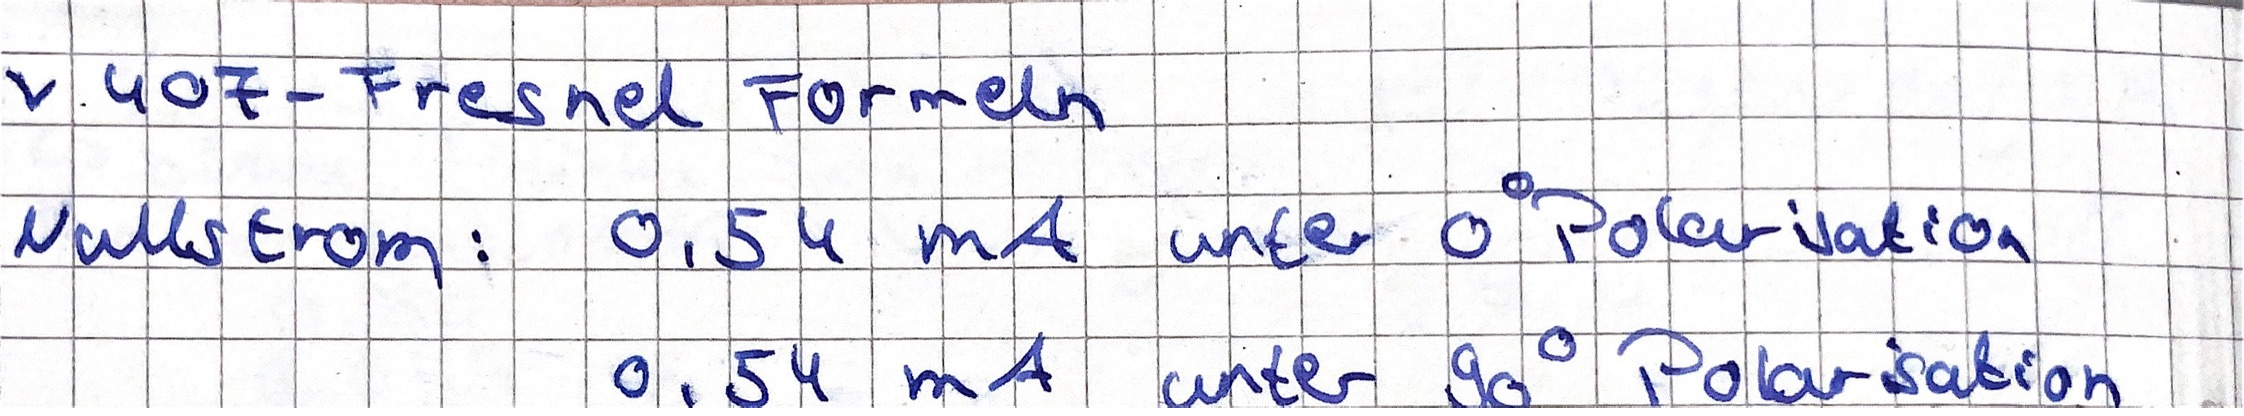
\includegraphics[width=0.5\textwidth]{data/origDaten1.png}
    \caption{Originale Messdaten.}
    \label{fig:origDaten1}
\end{figure}

\begin{figure}[H]
    \centering
    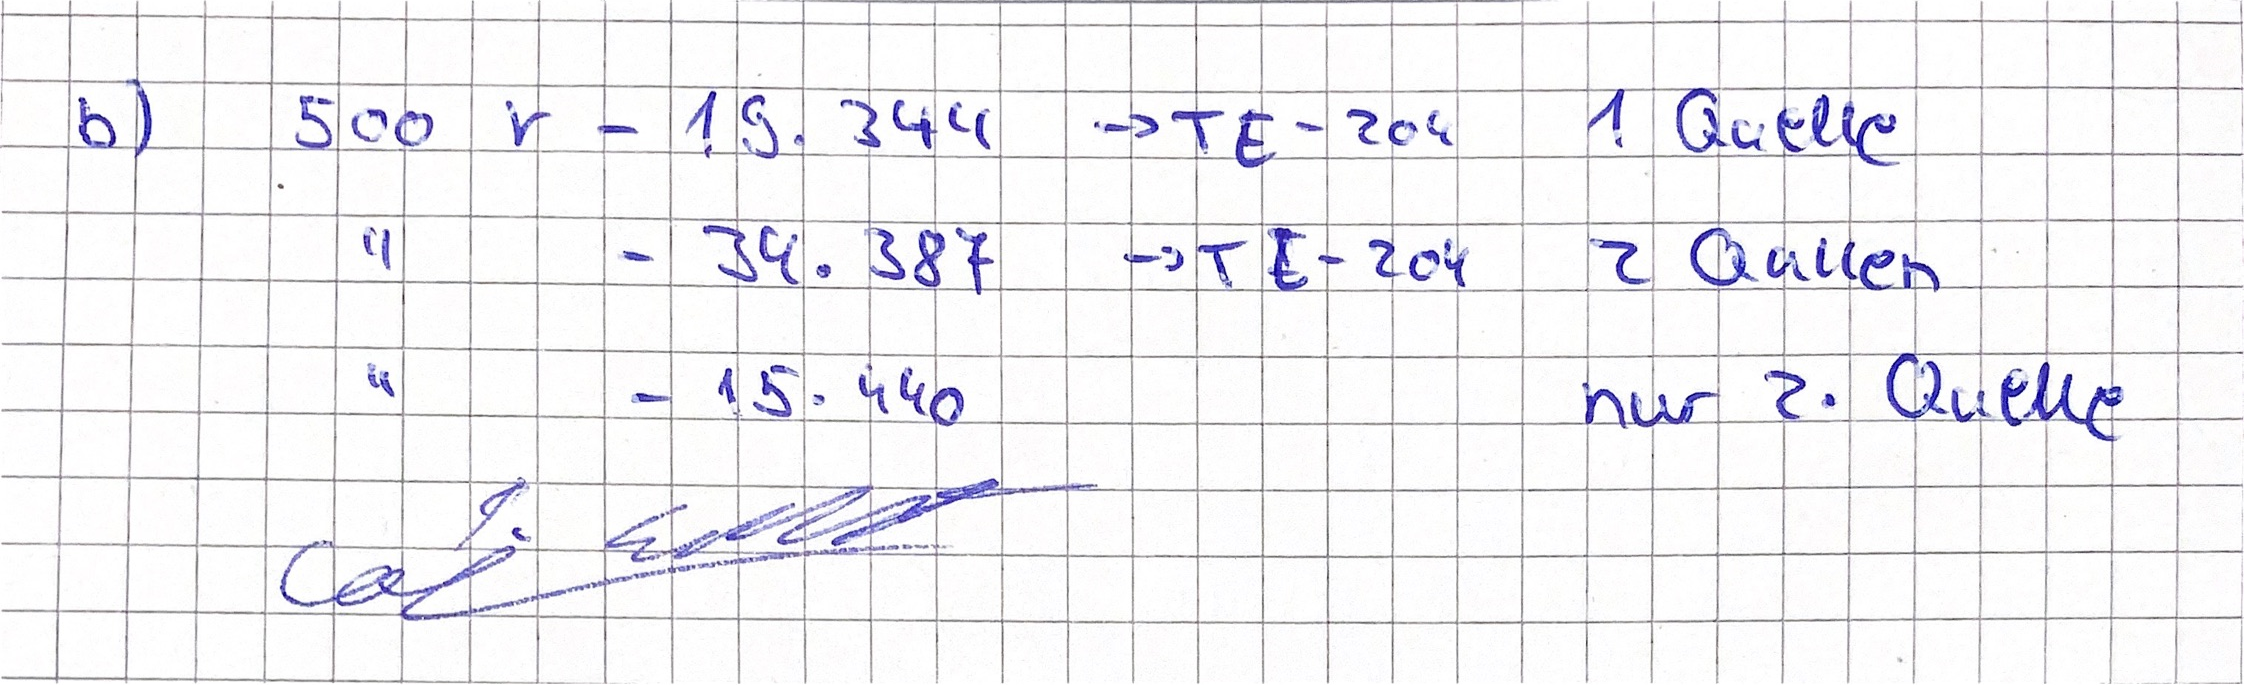
\includegraphics[width=0.5\textwidth]{data/origDaten2.png}
    \caption{Originale Messdaten.}
    \label{fig:origDaten2}
\end{figure}